%Lab Report
\documentclass[12pt,titlepage, a4paper]{article}
 \usepackage[german]{babel}
 \usepackage[utf8]{inputenc}
 \usepackage{graphicx}

\begin{document}

\title{Report\\Projektgruppe Kognitive Robotik}

\author{Münstermann,  Cedrick\\  Krombach, Nicola\\[1cm]
	Autonomous Intelligent Systems\\ \textsc{Universität Bonn}\\}



\maketitle


\section*{Abstract}


\section{Einleitung}

Im Rahmen der Projektgruppe Kognitive Robotik sollten in diesem Jahr die Aufgaben der European Robotics Challenges\footnote{http://www.euroc-project.eu/} bearbeitet werden. 
Die Aufgaben der European Robotics Challenges unterteilen sich dabei in drei Challenges, die wiederum verschiedene Unteraufgaben haben:

\begin{itemize}
 \item Challenge 1: Stationäre Manipulationsroboter in Kooperation mit Menschen (Track 1 \& 2)
 \item Challenge 2: Mobile Manipulationsroboter für die Logistik (Track 1 \& 2)
 \item Challenge 3: Flugroboter für industrielle Inspektion (Track 1 \& 2)
\end{itemize}

blabla mehr zu euroc? \\
Autonome Flugroboter eignen sich aufgrund ihres flexiblen Aufbaus und der Möglichkeit schwer zugängliche Objekte anzufliegen, besonders für die Inspektion und Überwachung von sehr großen industriellen
Anlagen oder Infrastrukturen. Dabei sollen sie autonom agieren, sodass auf die Abhängigkeit von einem Piloten verzichtet werden kann.
Auch für die Inspektion von gefährlichen Umgebungen eignet sich ein autonomer Flugroboter.

Unsere Gruppe befasste sich mit dem ersten Track der dritten Challenge, bei welchem die Lokalisierung des MAV und die 3D-Rekonstruktion der Umgebung mit Hilfe von Stereo-Bildern
im Vordergrund stand.



\section{Aufgabenstellung} 
In dem ersten Track von Challenge 3 geht es vorrangig um die Verarbeitung von visuellen Informationen, um die Pose des MAV zu schätzen und schließlich eine Karte von der Umgebung aufzubauen.



\subsection{Task 1 - Visuelle Lokalisierung}
In der ersten Aufgabe ging es darum aus Stereobildern eine 6D-Pose zu schätzen. Dazu wurden realistische Datensätze mit unterschiedlichen Schwierigkeiten zur Verfügung gestellt.
Ausschließlich anhand von diesen Datensätzen sollte nun die Lokalisierung erfolgen. Für die Evaluation war sowohl die lokale Genauigkeit als auch die Echtzeitfähigkeit der Berechnung entscheidend.
Eine \"Ubersicht der Evaluierungskriterien und Punktevergabe findet sich in \cite{eurocannex}.
Neben den Kamerabildern wurden zudem entsprechende Kalibrierungen des Kamerasystems und der IMU zur Verfügung gestellt. 
Für die Berechnung der visuellen Odometrie wurden zunächst zwei bereits in ROS verfügbare Verfahren getestet:\\
Das Paket Semi-direct Monocular Visual Odometry (SVO)\cite{EPFL-CONF-199740} und das Paket LIBVISO2 \cite{Geiger11}.
In ersten Experimenten stellte sich das LIBVISO2 als besser geeignet heraus, und zudem erlaubt es die Verwendung von Stereokameras für die visuelle Odometrie, 
im Gegensatz zu SVO, welches ein monokulares Verfahren ist.
Als Kamerakalibrierung wurde die bereitgestellte Kalibrierung mittels Aprilboard verwendet.
Da die Darstellung der Pose in IMU-Koordinaten erfolgen muss, rechnen wir die Pose mittels einer statischen Transformation aus der Kalibrierung von Kamerakoordinaten in IMU-Koordinaten um.
Die sich dadurch ergebende Transformationskette lautet:\\

$  map \rightarrow imu \rightarrow cam0 $\\

Da keine Groundtruth zur Verfügung gestellt wird, konnte man letztlich nur über die Online-Evaluation herausfinden, wie genau die berechnete Pose ist und wie hoch der relative Fehler ist.
Mit den Default-Werten von LIBVISO2 erhielten wir zu Beginn 4 Punkte bei der einfachsten Schwierigkeit. 
Davon 3 Punkte in der Genauigkeit mit einem mittleren relativen Translationsfehler von 2.6\% und 1 Punkt in der Laufzeit mit 105ms.
Die Laufzeit konnten wir mit dem Setzen des Compiler-Flags DCMAKE\_BUILD\_TYPE auf Release auf 39ms reduzieren, und erhielten so 3 Punkte in der Laufzeit.
Für die Erhöhung der Genauigkeit passten wir die Parameter von LIBVISO2 an die unterschiedlichen Schwierigkeiten an. 
So erhöhten wir den Parameter match\_radius von 100 auf 200 und die RANSAC-Iterationen von 150 auf 160.
Damit konnten wir den Fehler von 2.6\% auf 1.0\% reduzieren, und erhalten damit volle Punktzahl in der Genauigkeit.
Ein Beispiel einer solchen Evaluation ist in Abbildung~\ref{fig:evat1} zu sehen. Dort schneiden wir in der Genauigkeit sehr gut ab, mit einem gemittelten relativen Translationsfehler 
von 1\% erhalten wir für die Genauigkeit volle Punktzahl. Auch in der Laufzeit sind wir mit 40ms verhältnismäßig gut. Für die volle Punktzahl benötigt man eine Laufzeit kleiner 20ms.
Auch in der zweiten Schwierigkeitsstufe erhalten wir mit 8 von 10 möglichen Punkten ein gutes Ergebnis für die berechnete Odometrie. In der schwierigsten Stufe hat die visuelle Odometrie
jedoch einige Probleme die korrekte Pose zu schätzen, was durch die schlechteren Belichtungsverhältnisse und merkmalsärmere Umgebung zu erlären ist.
Wie in Abbildung~\ref{fig:evat3} zu sehen, driften wir vor allem in x- und y-Richtung stark.


\begin{figure}
 \centering
 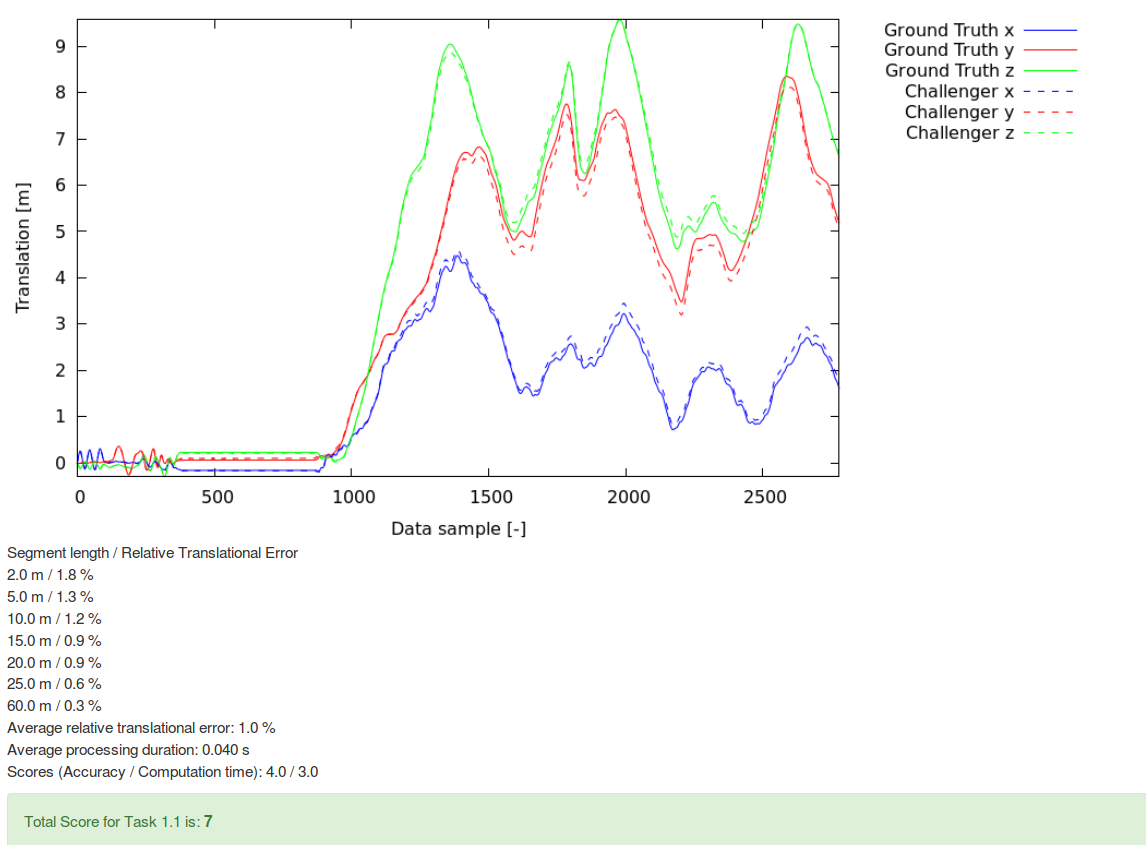
\includegraphics[width=\textwidth]{./Screens/t1_opt2_april.png}
 \caption{Ergebnis der Online-Evaluation zu Task 1.1 mit 7 von 8 möglichen Punkten} \label{fig:evat1}
\end{figure}
\begin{figure}
 \centering
 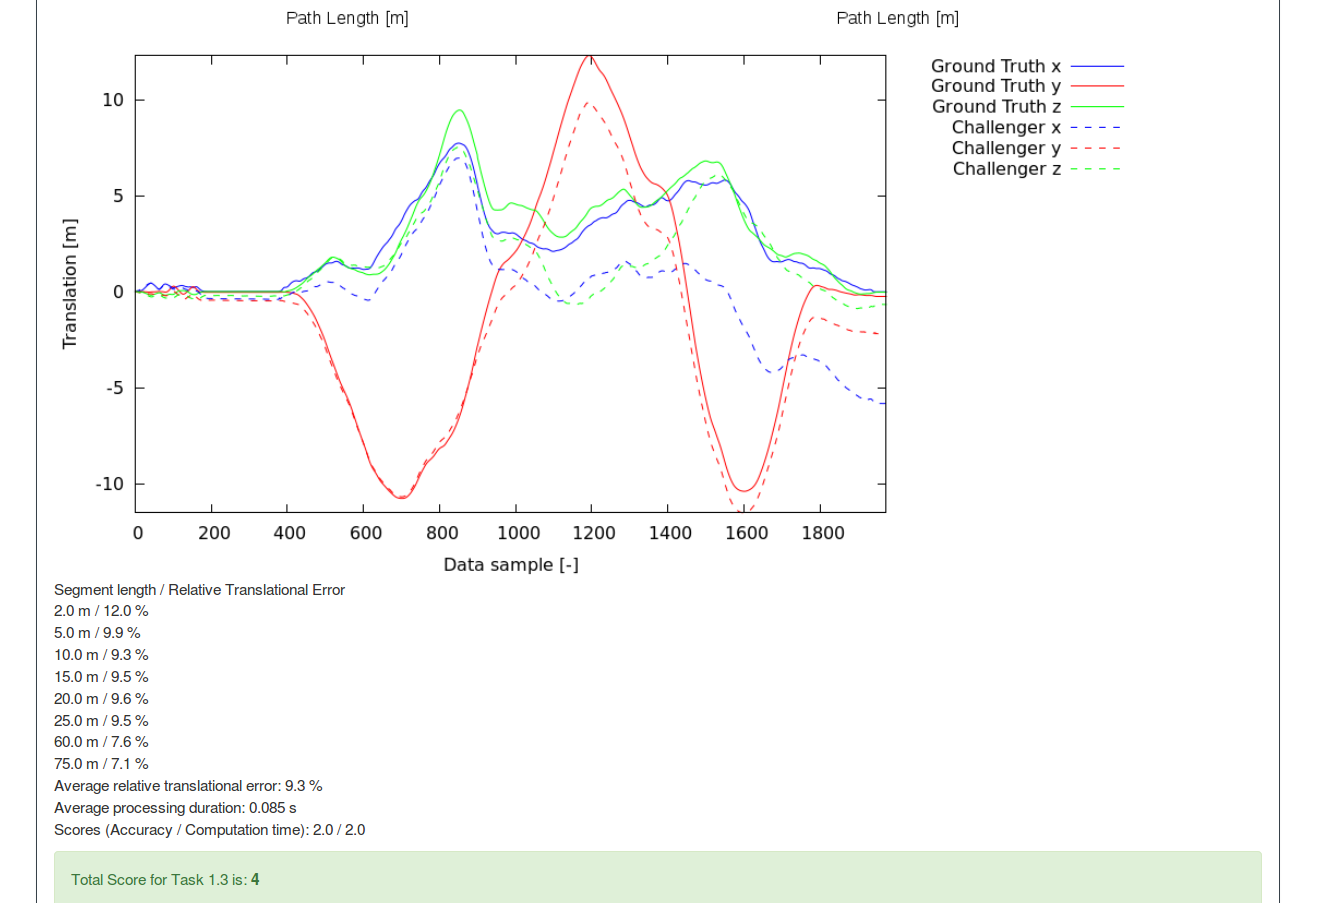
\includegraphics[width=\textwidth]{./Screens/t3_checkerboard.png}
 \caption{Ergebnis der Online-Evaluation zu Task 1.3 mit 5 von 8 möglichen Punkten} \label{fig:evat3}
\end{figure}


				
\subsection{Task 2 - 3D-Rekonstruktion}

Reconstruct environment in order to create a 3-D occupancy grid
Camera poses are given
create occupancy grid from depth images
Real-time computation, but over the whole dataset



\section{Experimente}




\section{Zusammenfassung}

  \bibliography{lit.bib}
  \bibliographystyle{alpha}
\end{document}
